\documentclass[border=5mm]{standalone}
\usepackage{pgfplots}
\usetikzlibrary{arrows.meta}
\pgfplotsset{compat=1.18}

\begin{document}
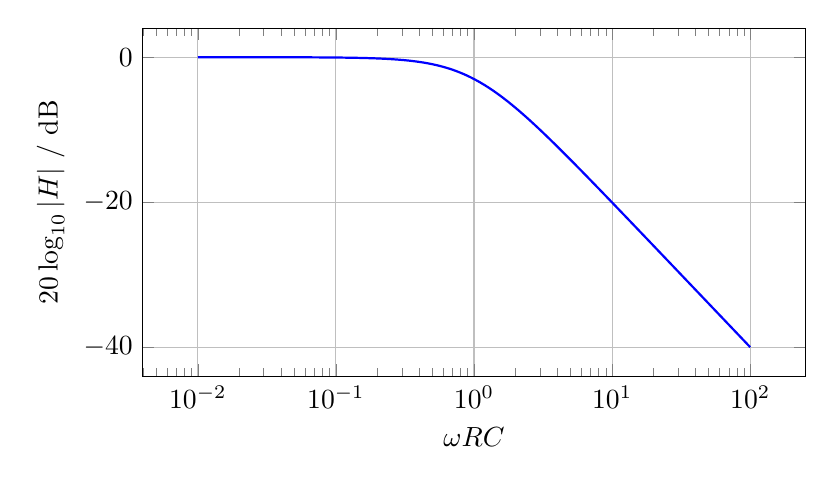
\begin{tikzpicture}[>=Stealth]
\begin{axis}[width=10cm,height=6cm,grid=major,xmode=log,xlabel={$\omega RC$},ylabel={$20\log_{10}|H|$ / dB}]
\addplot[blue,thick,domain=.01:100,samples=161]{-10*ln(1+x^2)/ln(10)};
\end{axis}
\end{tikzpicture}
\end{document}
